\section{The handoff}
\label{sec:handoff}

One OPX window per shot: ARTIQ triggers, turns its RF on for the OPX to gate,
and blocks until the OPX says it is done; then ARTIQ takes the RF back while
the OPX still holds the blocks. Four numbers govern it, all in
\code{ExptParams}:\footnote{\file{k-exp/kexp/config/expt\_params.py} lines
438--439, 455; \code{T\_OPX\_TRIGGER\_PULSE}/\code{T\_OPX\_HANDBACK\_TIMEOUT} in
\file{k-exp/kexp/base/control.py} lines 33--34.}

\begin{center}\small
\begin{tabular}{@{}llp{8.6cm}@{}}
\toprule
parameter & value & meaning \\
\midrule
\code{t\_opx\_handoff\_artiq\_side} & 350\nsu & trigger $\to$ ARTIQ RF on. \textbf{Unmeasured assumption} (M1): the OPX must have seen the trigger and raised its blocks by then \\
\code{t\_opx\_handoff\_opx\_side} & 1\us & RF-switch turn-off (MOSFET inverter) + ARTIQ DDS RF-switch rise time; ARTIQ returns to the caller at the sum, 1.35\us \\
\code{t\_opx\_handback\_overlap} & 15\us & OPX holds the blocks this long after its hand-back edge; ARTIQ takes the RF back at \emph{half} of it (7.5\us) \\
\code{T\_OPX\_TRIGGER\_PULSE} & 1\us & width of the ttl32 trigger pulse (cursor is rewound, so 0 timeline cost) \\
\code{T\_OPX\_HANDBACK\_TIMEOUT} & 2\,s & no edge by then $\to$ \code{TriggerTimeout} \\
\bottomrule
\end{tabular}
\end{center}

Decision D1 of the spec: the OPX settle wait is the \emph{sum}
\code{artiq\_side + opx\_side}, carried on the channel map as one field
\code{t\_handoff\_settle\_s} that \code{kexp\_channel\_map} fills with that
sum (\code{settle\_s = artiq\_side + opx\_side}, also recorded in the
machine's \code{extra}). Before the rebuild the map read a parameter
(\code{t\_opx\_handoff\_settle}) that commit \code{b77c728c} had replaced,
so every \code{self.opx.use(...)} died with \code{AttributeError} in
\code{prepare()}; the test fixtures fabricated the old name and passed.

\subsection{Timing diagram (a): as coded after the rebuild}
\label{sec:handoff:diag_a}

\begin{figure}[htbp]
\centering
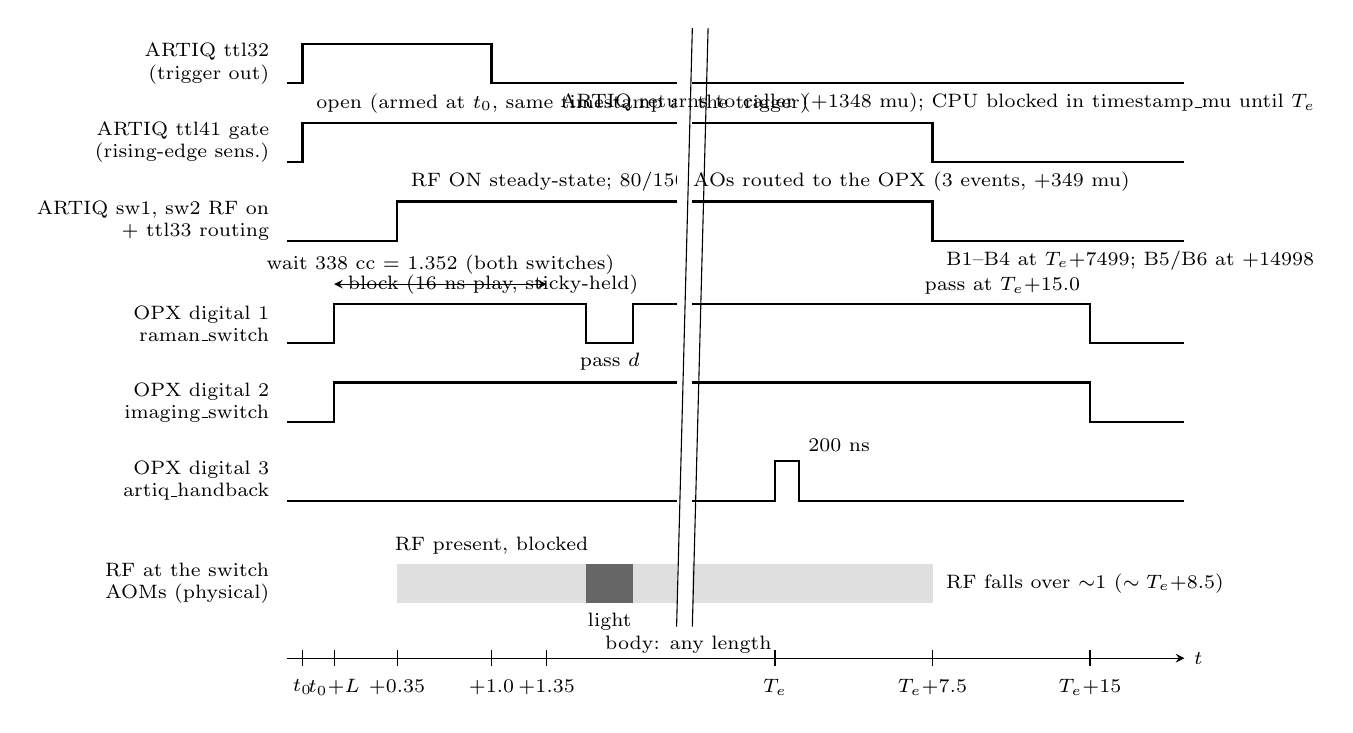
\begin{tikzpicture}[>=stealth, font=\scriptsize, x=1cm, y=1cm]
  % lane labels
  \node[anchor=east, align=right] at (0.7,6.25) {ARTIQ ttl32\\(trigger out)};
  \node[anchor=east, align=right] at (0.7,5.25) {ARTIQ ttl41 gate\\(rising-edge sens.)};
  \node[anchor=east, align=right] at (0.7,4.25) {ARTIQ sw1, sw2 RF on\\+ ttl33 routing};
  \node[anchor=east, align=right] at (0.7,2.95) {OPX digital 1\\\code{raman\_switch}};
  \node[anchor=east, align=right] at (0.7,1.95) {OPX digital 2\\\code{imaging\_switch}};
  \node[anchor=east, align=right] at (0.7,0.95) {OPX digital 3\\\code{artiq\_handback}};
  \node[anchor=east, align=right] at (0.7,-0.35) {RF at the switch\\AOMs (physical)};
  % ttl32: low 0.8-1.0, high 1.0-3.4, low after
  \draw[thick] (0.8,6.0) -- (1.0,6.0) -- (1.0,6.5) -- (3.4,6.5) -- (3.4,6.0) -- (12.2,6.0);
  % gate: open 1.0 -> 9.0
  \draw[thick] (0.8,5.0) -- (1.0,5.0) -- (1.0,5.5) -- (9.0,5.5) -- (9.0,5.0) -- (12.2,5.0);
  \node[anchor=south west] at (1.05,5.5) {open (armed at $t_0$, same timestamp as the trigger)};
  % sw/ttl33: high 2.2 -> 9.0
  \draw[thick] (0.8,4.0) -- (2.2,4.0) -- (2.2,4.5) -- (9.0,4.5) -- (9.0,4.0) -- (12.2,4.0);
  \node[anchor=south west] at (2.25,4.5) {RF ON steady-state; 80/150 AOs routed to the OPX (3 events, +349 mu)};
  \node[anchor=north west] at (9.05,4.0) {B1--B4 at $T_e$+7499; B5/B6 at +14998};
  % OPX digital 1: high 1.4 -> 4.6, low 4.6 -> 5.2 (exposure), high 5.2 -> 11.0
  \draw[thick] (0.8,2.7) -- (1.4,2.7) -- (1.4,3.2) -- (4.6,3.2) -- (4.6,2.7) -- (5.2,2.7) -- (5.2,3.2) -- (11.0,3.2) -- (11.0,2.7) -- (12.2,2.7);
  \node[anchor=south west] at (1.45,3.2) {block (16 ns play, sticky-held)};
  \node[anchor=north] at (4.9,2.7) {pass $d$};
  \node[anchor=south east] at (11.0,3.2) {pass at $T_e$+15.0\us};
  % OPX digital 2: high 1.4 -> 11.0
  \draw[thick] (0.8,1.7) -- (1.4,1.7) -- (1.4,2.2) -- (11.0,2.2) -- (11.0,1.7) -- (12.2,1.7);
  % OPX digital 3: pulse 7.0 -> 7.3
  \draw[thick] (0.8,0.7) -- (7.0,0.7) -- (7.0,1.2) -- (7.3,1.2) -- (7.3,0.7) -- (12.2,0.7);
  \node[anchor=south west] at (7.3,1.2) {200 ns};
  % physical RF: present 2.2 -> 9.0 (blocked), light 4.6 -> 5.2
  \fill[gray!25] (2.2,-0.6) rectangle (9.0,-0.1);
  \fill[black!60] (4.6,-0.6) rectangle (5.2,-0.1);
  \node[anchor=west] at (9.05,-0.35) {RF falls over $\sim$1\us\ ($\sim T_e$+8.5)};
  \node[anchor=south] at (3.4,-0.1) {RF present, blocked};
  \node[anchor=north] at (4.9,-0.6) {light};
  % settle bracket
  \draw[<->] (1.4,3.45) -- (4.1,3.45) node[midway, above] {wait 338 cc = 1.352\us\ (both switches)};
  % axis break
  \fill[white] (5.75,-0.9) rectangle (5.95,6.7);
  \draw (5.75,-0.9) -- (5.95,6.7);
  \draw (5.95,-0.9) -- (6.15,6.7);
  \node[anchor=north] at (5.9,-0.9) {body: any length};
  % time axis
  \draw[->] (0.8,-1.3) -- (12.2,-1.3) node[right] {$t$};
  \foreach \x/\lab in {1.0/$t_0$, 1.4/$t_0{+}L$, 2.2/+0.35\us, 3.4/+1.0\us, 4.1/+1.35\us, 7.0/$T_e$, 9.0/$T_e{+}7.5\us$, 11.0/$T_e{+}15\us$} {
    \draw (\x,-1.4) -- (\x,-1.2);
    \node[anchor=north] at (\x,-1.45) {\lab};
  }
  % ARTIQ CPU state
  \node[anchor=north west] at (4.15,6.0) {ARTIQ returns to caller (+1348 mu); CPU blocked in \code{timestamp\_mu} until $T_e$};
\end{tikzpicture}
\caption{The handshake as coded after the rebuild, one shot. $t_0$ is the
RTIO timestamp of the ttl32 rising edge; $L$ is the OPX trigger-to-output
latency, which QM does not publish; $T_e$ is the gateware timestamp of the
hand-back edge. ARTIQ numbers: \code{seconds\_to\_mu} floors, so 350\nsu\ $\to$
349\,mu, 1\us\ $\to$ 999\,mu, 7.5\us\ $\to$ 7499\,mu. OPX numbers: 338 and
3750\,cc. Sources: \file{k-exp/kexp/base/control.py}
\code{handoff\_to\_quantum\_machines} / \code{wait\_for\_quantum\_machines\_handback};
\file{wax/waxx-src/waxx/control/artiq/TTL.py} \code{arm} / \code{wait\_for\_edge};
\file{k-exp/kexp/control/opx/builder.py} \code{trace};
\file{context.py} \code{handback\_to\_artiq}.}
\label{fig:timing_a}
\end{figure}

\paragraph{The ARTIQ event list, exactly.} With $t_0$ = the trigger edge
(\code{t\_trigger = now\_mu()}), all times in mu (= ns):

\begin{center}\small
\begin{tabular}{@{}llll@{}}
\toprule
\# & $t$ (rel.\ $t_0$) & channel & event \\
\midrule
A0 & -- & ttl41 FIFO & \code{clear\_input\_events(0)}: non-blocking drain of stale edges (CPU only) \\
A1 & 0 & ttl41 sensitivity & \code{\_set\_sensitivity(1)}: gate open \\
A2 & 0 & ttl32 & trigger HIGH \\
A3 & +999 & ttl32 & trigger LOW (\code{pulse(1e-6)}) \\
-- & cursor $\to$ 0, then $+349$ & & \code{at\_mu(t\_trigger)}; \code{delay(t\_opx\_handoff\_artiq\_side)} \\
A4 & +349 & ttl33 & routing HIGH: 80/150 AOs now driven by the OPX \\
A5 & +349 & \code{ttl\_urukul5\_sw2} & \code{imaging.on()} $\to$ one RTIO switch write (no DAC on this DDS) \\
A6 & +349 & \code{ttl\_urukul5\_sw1} & \code{raman.on()} $\to$ one RTIO switch write \\
-- & cursor $\to$ +1348 & & \code{delay(t\_opx\_handoff\_opx\_side)}; return to the caller \\
-- & & & \code{wait\_for\_edge(7.5e-6, 2.)}: CPU blocks in \code{timestamp\_mu} \\
B1 & $T_e$+7499 & ttl41 sensitivity & gate closed \\
B2 & $T_e$+7499 & \code{sw2} & imaging switch RF OFF (\code{dds\_sw.set\_sw(0)}) \\
B3 & $T_e$+7499 & \code{sw1} & raman switch RF OFF \\
B4 & $T_e$+7499 & ttl33 & routing LOW: AOs back on the ARTIQ DDSs \\
-- & (VERBOSE) & & \code{aprint} of the slack left: \emph{the M1 measurement of the CPU reaction time} \\
B5, B6 & $T_e$+14998 & \code{sw2}, \code{sw1} & \code{imaging.off()}, \code{raman.off()}: re-assert the level (redundant, kept for bookkeeping) \\
\bottomrule
\end{tabular}
\end{center}

Three corrections to older docstrings, now written into
\code{control.py}'s two kernels: the RF-off events and the ttl33 drop carry
the \emph{same} timestamp (there is no ``RF off before the TTL drops''
ordering; it is harmless because the switch AOM is blocked until
$T_e$+15\us); the ``full \code{off()} is several SPI writes'' rationale does
not apply -- these two DDSs have no DAC channel, so \code{on()}/\code{off()}
are one RTIO write each; and the crash state is not ``blocks left HIGH''
(section~\ref{sec:handoff:crash}). The comment block above the parameters in
\file{expt\_params.py} (lines 431--461) has been rewritten to the same
contract: the block-before-RF ordering is labelled ``ASSUMPTION, NOT
MEASURED (milestone M1)'', the settle is the sum, the take-back is
switch-only, and the parameters are marked config-time.

\paragraph{The hand-back slot.} Between $T_e$ and $T_e$+7499\,mu the kernel
CPU must wake from \code{timestamp\_mu} (the repo's own estimate: $\sim$3\us),
and submit four events ($\sim$0.5--1\us\ each). Need 5--7\us\ against
7.5\us\ available. The old \code{TTL.py} docstring asked for $\ge 10\us$; it
now says ``keep it comfortably above [the kernel CPU's reaction time]. It
has not been measured on this machine: $\sim$4--7\us\ is expected, and
\code{Control.wait\_for\_quantum\_machines\_handback} prints the slack left
after its critical events at VERBOSE -- that print is the measurement.'' An
underflow here is caught by \code{scan()} and aborts the run.

\subsection{Timing diagram (b): the customer 00e-era script, for comparison}
\label{sec:handoff:diag_b}

The 30-shot \file{customer-weld-ucsb/experiments/00e\_hello\_atoms\_scan.py}
was run (by file mtime) against the ARTIQ of commits
\code{063c3b07}/\code{612698b9}: RF on at \code{t\_opx\_handoff\_settle/2} =
5\us, take-back at \code{overlap/2} = 5\us\ (overlap 10\us).\footnote{Phase-1
report \code{customer\_handoff.md} \S0 and \S2.3; \code{git show 063c3b07:kexp/base/control.py}.}

\begin{figure}[htbp]
\centering
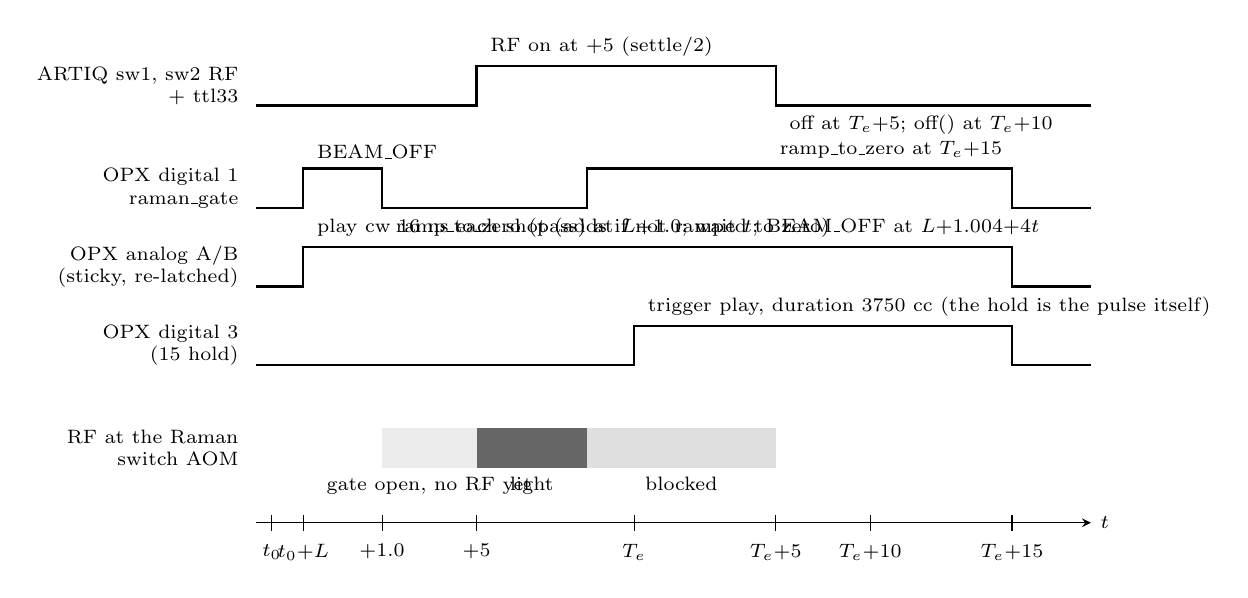
\begin{tikzpicture}[>=stealth, font=\scriptsize, x=1cm, y=1cm]
  \node[anchor=east, align=right] at (0.7,4.25) {ARTIQ sw1, sw2 RF\\+ ttl33};
  \node[anchor=east, align=right] at (0.7,2.95) {OPX digital 1\\\code{raman\_gate}};
  \node[anchor=east, align=right] at (0.7,1.95) {OPX analog A/B\\(sticky, re-latched)};
  \node[anchor=east, align=right] at (0.7,0.95) {OPX digital 3\\(15\us\ hold)};
  \node[anchor=east, align=right] at (0.7,-0.35) {RF at the Raman\\switch AOM};
  % ARTIQ RF: on at 3.6 (+5us), off at 7.4 (Te+5)
  \draw[thick] (0.8,4.0) -- (3.6,4.0) -- (3.6,4.5) -- (7.4,4.5) -- (7.4,4.0) -- (11.4,4.0);
  \node[anchor=south west] at (3.65,4.5) {RF on at +5\us\ (settle/2)};
  \node[anchor=north west] at (7.45,4.0) {off at $T_e$+5\us; off() at $T_e$+10};
  % raman_gate: BEAM_OFF at L (1.4), ramp_to_zero at 2.4 (L+1.0us), BEAM_OFF at 5.0, ramp_to_zero at 10.4 (Te+15)
  \draw[thick] (0.8,2.7) -- (1.4,2.7) -- (1.4,3.2) -- (2.4,3.2) -- (2.4,2.7) -- (5.0,2.7) -- (5.0,3.2) -- (10.4,3.2) -- (10.4,2.7) -- (11.4,2.7);
  \node[anchor=south west] at (1.45,3.2) {BEAM\_OFF};
  \node[anchor=north west] at (2.45,2.7) {ramp\_to\_zero (pass) at $L$+1.0\us; wait $t$; BEAM\_OFF at $L$+1.004\us+4$t$};
  \node[anchor=south east] at (10.4,3.2) {ramp\_to\_zero at $T_e$+15\us};
  % analog: latch at 1.4, ramp_to_zero at 10.4
  \draw[thick] (0.8,1.7) -- (1.4,1.7) -- (1.4,2.2) -- (10.4,2.2) -- (10.4,1.7) -- (11.4,1.7);
  \node[anchor=south west] at (1.45,2.2) {play cw 16 ns each shot (adds if not ramped to zero)};
  % digital 3: 5.6 -> 10.4
  \draw[thick] (0.8,0.7) -- (5.6,0.7) -- (5.6,1.2) -- (10.4,1.2) -- (10.4,0.7) -- (11.4,0.7);
  \node[anchor=south west] at (5.65,1.2) {trigger play, duration 3750 cc (the hold is the pulse itself)};
  % physical: gate open no RF 2.4 -> 3.6 (hatched-ish: lighter), light 3.6 -> 5.0
  \fill[gray!15] (2.4,-0.6) rectangle (3.6,-0.1);
  \fill[black!60] (3.6,-0.6) rectangle (5.0,-0.1);
  \fill[gray!25] (5.0,-0.6) rectangle (7.4,-0.1);
  \node[anchor=north] at (3.0,-0.6) {gate open, no RF yet};
  \node[anchor=north] at (4.3,-0.6) {light};
  \node[anchor=north] at (6.2,-0.6) {blocked};
  \draw[->] (0.8,-1.3) -- (11.4,-1.3) node[right] {$t$};
  \foreach \x/\lab in {1.0/$t_0$, 1.4/$t_0{+}L$, 2.4/+1.0\us, 3.6/+5\us, 5.6/$T_e$, 7.4/$T_e{+}5\us$, 8.6/$T_e{+}10\us$, 10.4/$T_e{+}15\us$} {
    \draw (\x,-1.4) -- (\x,-1.2);
    \node[anchor=north] at (\x,-1.45) {\lab};
  }
\end{tikzpicture}
\caption{The 00e-era handoff. The OPX opened the Raman gate at $t_0 + L +
1.0\us$ but ARTIQ's RF reached the switch AOM only at $t_0 + 5\us$: the first
$4\us - L$ of every exposure had no RF, and the four shortest non-zero
settings (1.07, 2.14, 3.21, 4.28\us) produced no light at all (inferred; it
holds if the committed \code{control.py} was the one running). Also visible:
the 15\us\ hold is the trigger \emph{pulse} itself, the blocks are released by
the sticky end-of-statement rule rather than an explicit pass, the analog
drives are re-latched every shot (safe only because of the trailing
\code{ramp\_to\_zero}), and each exposure carries the 4\nsu\ ramp. Source:
\file{00e\_hello\_atoms\_scan.py} lines 47--94, \file{configuration.py}.}
\label{fig:timing_b}
\end{figure}

What the builder changed relative to 00e: exposure is a \code{pass} play of
exactly $d$ (no ramp, no $+4\nsu$); the analog drives are latched once per
run; the blocks idle low between shots; the hand-back trigger is 200\nsu\
and the hold is a \code{wait} on the switch elements; and the shot values
come from the same shuffled tables as the ARTIQ scan instead of an OPX-side
list that the HDF5 file knew nothing about.

\subsection{Waste and risk, per OPX window}
\label{sec:handoff:waste}

\begin{table}[htbp]
\centering
\scriptsize
\begin{tabular}{@{}llp{7.6cm}l@{}}
\toprule
\# & item & detail & kind \\
\midrule
W1 & overlap 15\us\ vs $\sim$8.5--10\us\ need & CPU reaction ($\sim$4--7\us) + RF fall ($\sim$1\us) + margin; $\sim$5\us\ idle per window, 15\us\ dead on the ARTIQ timeline & waste \\
W2 & handoff settle & 1.35\us\ dead time both sides; the 00e script waited 9.984\us & waste \\
W3 & B5/B6 & two RTIO writes re-asserting a level written 7.5\us\ earlier (\code{off()} bookkeeping) & waste \\
W4 & 2\,s timeout & with a dead job every shot burns 2\,s \textbf{with both switch-AOM RFs ON and the OPX lines idle low (= pass)}: light on the atoms and detector until \code{TriggerTimeout} & waste + physics \\
W5 & aligns & the removed A2 and the trailing \code{wait\_s} align cost a few cycles each & negligible \\
W6 & both RFs on regardless of claims & \code{handoff\_to\_quantum\_machines} turns raman \emph{and} imaging RF on unconditionally, so both blocks are guarded in every window; a raman-only sequence still blocks the imaging switch & design \\
W7 & imaging intensity servo & whether it winds up while its switch is blocked depends on where its photodiode sits; PID clear/override TTLs are dead; M1 & risk (open) \\
W8 & \code{prep\_raman} & 10.7--28.2\,ms per shot (warm-up, shutter, line trigger); necessary, dwarfs W1/W2 & info \\
R1 & handoff leak & ARTIQ RF at +349\,mu vs block complete at $L$ + align + $\sim$1\us\ turn-off: \textbf{up to $\sim$0.65--1\us\ of raman and imaging light} if $L \sim 1\us$; unmeasured & logic-risk \\
R2 & take-back CPU margin & 0.5--3.5\us\ depending on which in-repo per-event cost is right & logic-risk \\
R3 & underflow in the take-back left RF on & fixed: \code{cleanup\_scan\_kernel} now calls \code{imaging.off()}, \code{raman.off()} (\file{base.py} lines 311--316) & fixed \\
R4 & crash left ttl33 HIGH into the next run & fixed: \code{init\_kernel} drops ttl33 after \code{switch\_all\_dds(0)} (\file{base.py} line 180) & fixed \\
R5 & crash-state docstrings & rewritten in \code{control.py} (section~\ref{sec:handoff:crash}), in \code{TTL.py} (\code{wait\_for\_edge}) and in the \code{expt\_params.py} comment block & doc \\
R6 & 00e sticky release timing & the 00d/00f single-shot release relies on the end-of-program ramp & inferred \\
\bottomrule
\end{tabular}
\caption{Waste and risk items from the phase-1 handshake audits
(\code{artiq\_handshake.md} \S4, \code{customer\_handoff.md} \S3).}
\label{tab:waste}
\end{table}

\subsection{Unmeasured assumptions (the M1 list)}
\label{sec:handoff:m1}

Everything below must be seen on a scope with no atoms before this design
is trusted:

\begin{enumerate}[nosep]
  \item Trigger $\to$ block-complete latency versus the 350\nsu\ assumption.
    Both beams leak if it fails (R1). The previous design (RF at settle/2 =
    5\us) was safe by construction; the current one is faster and unproven.
  \item Hand-back CPU slack: the VERBOSE \code{aprint} in
    \code{wait\_for\_quantum\_machines\_handback} is the measurement and has
    never been run. Expected 4--7\us\ against the 7.5\us\ slot.
  \item Digital line state after \code{job.halt()} mid-block. If a line stays
    HIGH, every following non-OPX run has that switch AOM's RF blocked.
  \item QOP acceptance of port-less sticky digital elements
    (\code{raman\_switch}/\code{imaging\_switch} have no analog port). If
    refused, add the dummy analog port as QM's template did.
  \item Run once with \emph{no} OPX job: every shot must end in
    \code{TriggerTimeout}, never in a false edge on ttl41.
  \item Whether the sticky analog hold keeps the IF tone \emph{oscillating}
    (the lab saw RF on the AOs in 00d/00e, so empirically yes; one explicit
    trace).
  \item The imaging intensity servo while its switch is blocked (W7).
\end{enumerate}

\subsection{End states on crash and abort (corrected)}
\label{sec:handoff:crash}

The old docstrings said an ARTIQ crash mid-window ``leaves the blocks HIGH
until the ARTIQ process exits''. That is not what the emitted program does:
after \code{wait\_for\_trigger} the OPX shot has no further dependency on
ARTIQ -- body, A4, 200\nsu\ trigger, \code{wait(3750)}, \code{pass} -- so the
blocks are released 15\us\ after every hand-back whatever ARTIQ does.

\begin{center}\small
\begin{tabular}{@{}p{4.2cm}p{10.4cm}@{}}
\toprule
case & end state \\
\midrule
ARTIQ underflows \emph{before} the handoff & no trigger; OPX parked at \code{wait\_for\_trigger} with blocks at pass; \code{cleanup\_scan\_kernel} drops ttl33; \code{end()} $\to$ \code{finish()} halts the job. Safe. \\
ARTIQ underflows \emph{between} handoff and hand-back & the OPX finishes its shot and releases the blocks at $T_e$+15\us; ARTIQ never runs the take-back. Before the rebuild the raman and imaging RF stayed ON (cleanup only dropped ttl33 and the shutter) and imaging light passed until the next run's \code{init\_kernel}. Now \code{cleanup\_scan\_kernel} also calls \code{imaging.off()} and \code{raman.off()} (one RTIO event each). \\
Hand-back never comes (dead job) & \code{TriggerTimeout} after 2\,s (below); blocks are whatever the dead job left -- HIGH if it died mid-body, until halt. \\
Kernel dies while blocked (uncaught exception, \code{TerminationRequested} from a liveOD abort) & \textbf{the real crash end state:} ARTIQ RF ON on both switch AOMs, ttl33 HIGH, OPX blocks LOW after $T_e$+15\us, OPX tones still on the AOs until the \code{atexit} halt. Raman + imaging light pass until the next run's \code{init\_kernel} (\code{switch\_all\_dds(0)}); before the rebuild that run's first shot also ran with ttl33 HIGH -- the 80/150 AOs routed to a halted OPX, i.e.\ no Raman RF -- until its first \code{cleanup\_scan\_kernel}. Now \code{init\_kernel} drops ttl33 right after \code{switch\_all\_dds(0)}. \code{analyze()} never runs, so \code{finish()} never fetches: OPX data of such a run is lost (the underflow/timeout paths preserve it). \\
\code{scan(raise\_underflow=True)} & no cleanup at all: coils hot, RF on, ttl33 high. Not for use with atoms. \\
\bottomrule
\end{tabular}
\end{center}

\subsection{The \code{TriggerTimeout} path}

\code{wait\_for\_edge(7.5e-6, 2.)} computes \code{t\_deadline = now\_mu() +
seconds\_to\_mu(2.)} and blocks in \code{timestamp\_mu(t\_deadline)}. With no
edge it returns $-1$ after 2.0000013\,s; the cursor is placed at
\code{t\_deadline + 7499}, B1--B4 are written (positive slack $\sim$7.4\us),
then B5/B6, then \code{aprint} and \code{raise TriggerTimeout}. \code{Scanner.scan}
catches it (an own \code{except} clause: the compiler gives a local one type,
so it cannot share the underflow handler's name), runs
\code{cleanup\_scan\_kernel}, sets \code{aborted\_bool}, and ends the run with
the shots taken; with \code{save\_on\_underflow=True} \code{analyze()} still
runs, \code{finish()} fetches what the job streamed, and the missing shots are
NaN with \code{opx\_data\_valid = 0}. The physics cost is W4: 2\,s of light per
failing shot. A shorter timeout (0.2\,s) was recommended; the only legitimately
long OPX body is a feedback loop, and that is 1--2\,ms.
